\documentclass[__main__.tex]{subfiles}

\begin{document}

\qtitle{С}{06}
Потенциал электростатического поля, эквипотенциальные поверхности. Вычисление потенциала по известной напряжённости поля и определение конфигурации поля по заданному потенциалу.\\ 

\begin{definition}
Электростатический потенциал — скалярная энергетическая характеристика электростатического поля, характеризующая потенциальную энергию, которой обладает единичный положительный пробный заряд, помещённый в данную точку поля.$$\phi = \phi(x,y,z)$$
\end{definition}
Так же, надо отметить, что потенциал определен с точностью до константы $\phi ' = \phi + C$.\\
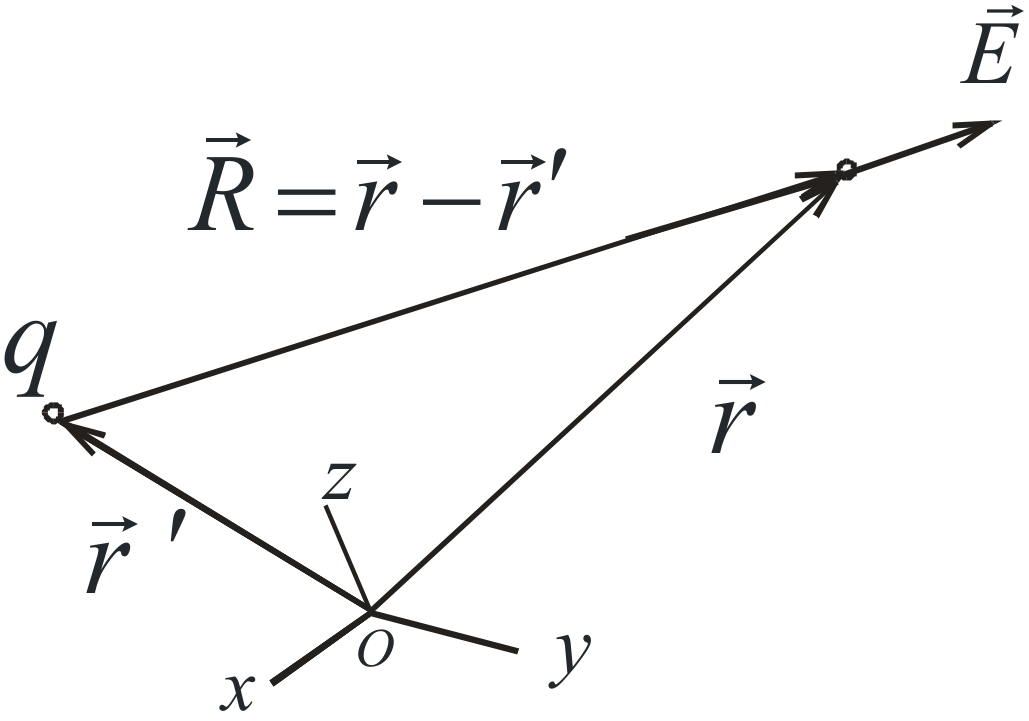
\includegraphics[scale = 0.3]{C6_1}\\
Итак, мы знаем как выражается напряженность $\vec{E} = -\nabla \phi$.\\
Тогда, мы в состоянии найти потенциал по известной напряженности поля:\\
\begin{gather}
\vec{E} = k\frac{q}{R}\frac{\vec{R}}{R} = k \frac{q}{|\vec{r}-\vec{r}'|2}\frac{\vec{r}-\vec{r}''}{|\vec{r}-\vec{r}'|} = -\nabla_{\vec{r}}\left(k\frac{q}{|\vec{r}-\vec{r}'|}+C\right),\\
\phi = k \frac{q}{|\vec{r}-\vec{r}'|}+C,
\end{gather}
где $k = \frac{1}{4 \pi \epsilon_0}$.\\
Если $\phi(\infty) = 0$, то $C = 0$.\\
\begin{gather}
\phi = k\frac{q}{R}
\end{gather}
Если же мы знаем потенциал $\phi = k \frac{q}{|\vec{r}-\vec{r}'|}$, то из определения $\vec{E} = - \nabla \phi$ получим:
\begin{gather}
\vec{E} = - \nabla \phi = - \nabla_{\vec{r}}\left(k \frac{q}{|\vec{r}-\vec{r}'|}\right) = k\frac{q}{|\vec{r}-\vec{r}'|^2}\frac{\vec{r}-\vec{r}'}{|\vec{r}-\vec{r}'|} = k\frac{q}{R^2}\frac{\vec{R}}{R}
\end{gather}
\begin{definition}
Эквипотенциальной поверхностью, или поверхностью равного потенциала, является поверхность, для любых точек которой разность потенциалов равна нулю. Это означяет, что работа по перемещению заряда по такой поверхности равна нулю, следовательно, линии напряженности электрического поля перпендикулярны эквипотенциальным поверхностям.$$\phi = \phi(x,y,z) = const$$
\end{definition}

\end{document}